\section{Experiments}
\label{sec:experiments}

We evaluate \ours on LiveQA-Bench (our streaming QA benchmark) and compare against published results on OVO-Bench~\cite{li2025ovobench}. We reference standard results on NExT-QA and EgoSchema, ablate each component, and profile per-query latency.

\subsection{Benchmarks}
\label{sec:benchmarks}

\paragraph{OVO-Bench.}
OVO-Bench~\cite{li2025ovobench} is an online video understanding benchmark from CVPR~2025.
It provides 644 videos with 2,814 multi-choice questions under causal constraints, organized into backward tracing (BT), real-time visual perception (RT), and forward active response (FA).
We report published results from~\cite{li2025ovobench} to establish the current state of streaming video understanding.

\paragraph{NExT-QA and EgoSchema (reference).}
NExT-QA~\cite{xiao2021nextqa} (52K QA pairs, 5,440 clips, avg.\ 44\,s) tests causal and temporal reasoning.
EgoSchema~\cite{mangalam2023egoschema} (5K multiple-choice questions, 3-minute Ego4D clips) targets long-form egocentric video understanding.
We reference published full-video results on these benchmarks to contextualize \ours within the broader VideoQA landscape.

\paragraph{LiveQA-Bench (ours).}
We built LiveQA-Bench to test temporal reasoning under streaming constraints, filling a gap left by existing benchmarks that assume full video access.
It contains 50 simulated live streams (5 to 30 minutes each), constructed by joining Ego4D~\cite{grauman2022ego4d} and Kinetics clips with natural transitions.
500 questions (10 per stream) span three temporal scopes, each with distinct reasoning requirements:

\begin{itemize}[itemsep=1pt,leftmargin=*]
  \item \textbf{Instantaneous} (170 Qs): targets the present frame---\emph{``What is happening right now?''}, \emph{``Is anyone in the scene?''}. Answerable from the latest keyframe alone.
  \item \textbf{Recent} (180 Qs): targets the last 30\,s---\emph{``What just happened?''}, \emph{``What was the person doing recently?''}. Requires aggregating a short window of context.
  \item \textbf{Historical} (150 Qs): targets the full stream---\emph{``How many different scenes have appeared?''}, \emph{``Did anything change earlier?''}. Requires long-range memory over the entire video.
\end{itemize}

\noindent Each question carries a ground-truth answer and a scope label.
Metrics are overall accuracy and per-scope accuracy.
\Cref{tab:bench_compare} situates LiveQA-Bench among related benchmarks.
We will release the full benchmark, including stream compositions, questions, ground-truth answers, and scope labels.

\begin{table}[t]
  \caption{\textbf{Benchmark comparison.} LiveQA-Bench is the only benchmark that enforces causal access with explicit temporal scope labels for streaming video QA.}
  \label{tab:bench_compare}
  \centering
  \small
  \setlength{\tabcolsep}{2.5pt}
  \begin{tabular}{@{}lccccc@{}}
    \toprule
    Benchmark & Videos & QA Pairs & Dur.\ (s) & Scope & Causal \\
    \midrule
    NExT-QA~\cite{xiao2021nextqa}       & 5{,}440 & 52K   & 44  & \xmark & \xmark \\
    EgoSchema~\cite{mangalam2023egoschema} & 5{,}000 & 5K  & 180 & \xmark & \xmark \\
    OVO-Bench~\cite{li2025ovobench}      & 644     & 2.8K  & var & \cmark & \cmark \\
    \midrule
    \textbf{LiveQA-Bench}                & 50      & 500   & 300--1800 & \cmark & \cmark \\
    \bottomrule
  \end{tabular}
\end{table}

\subsection{Baselines}
\label{sec:baselines}

\paragraph{Streaming video models.}
Three recent streaming models serve as primary baselines:
\textbf{Flash-VStream}~\cite{zhang2024flashvstream} (memory-based real-time understanding),
\textbf{VideoLLM-online}~\cite{chen2024videollmonline} (online decoding), and
\textbf{Dispider}~\cite{he2024dispider} (disentangled perception-decision-reaction).
On OVO-Bench we report results published by Li~et~al.~\cite{li2025ovobench}.

\paragraph{Offline video models.}
For LiveQA-Bench we additionally evaluate five offline models adapted to streaming (frames up to $t_q$ only):
\textbf{Video-ChatGPT}~\cite{maaz2023videochatgpt},
\textbf{VideoLLaVA}~\cite{lin2023videollava},
\textbf{SeViLA}~\cite{yu2023sevila},
\textbf{LLaVA-Next-Video}~\cite{zhang2024llavanextvideo},
\textbf{Chat-UniVi}~\cite{jin2024chatunivi},
and \textbf{LLaVA-NV + Buffer} (LLaVA-Next-Video with a FIFO buffer of $N\!=\!64$).
For OVO-Bench we include published results for \textbf{Qwen2-VL-7B}~\cite{wang2024qwen2vl} and \textbf{LLaVA-OneVision-7B}~\cite{li2024llavaonevision} as offline upper bounds.

\paragraph{Implementation details.}
\ours uses CLIP ViT-B/32 as the vision encoder, BLIP-base for captioning and VQA, and Flan-T5-base as the language synthesis model.
We resize input frames to $224\times224$ for CLIP and $384\times384$ for BLIP. Memory capacity $N\!=\!64$. TQR recent window $W\!=\!30$\,s.
All \ours results on LiveQA-Bench are measured on an NVIDIA T4 GPU (Google Colab).


\subsection{Main Results}

\paragraph{OVO-Bench.}
\Cref{tab:ovobench} shows published results on OVO-Bench~\cite{li2025ovobench}.
A large gap persists between offline models with full video access and streaming models restricted to causal processing.
Among streaming methods, Dispider~\cite{he2024dispider} leads with 41.8\% overall, followed by Flash-VStream~\cite{zhang2024flashvstream} at 33.6\%; VideoLLM-online~\cite{chen2024videollmonline} fails to complete forward-active tasks.
Backward tracing is the weakest category for all streaming models, confirming that long-range memory under causal constraints remains an open challenge---the gap that \ours targets with importance-scored keyframe retention and temporal routing.

\begin{table}[t]
  \caption{\textbf{OVO-Bench results} (published~\cite{li2025ovobench}). Accuracy (\%) per category: Backward Tracing (BT), Real-Time Perception (RT), Forward Active Response (FA). All numbers from Li~et~al.; streaming models use causal access only.}
  \label{tab:ovobench}
  \centering
  \small
  \setlength{\tabcolsep}{3pt}
  \begin{tabular}{@{}lcccc@{}}
    \toprule
    Method & BT & RT & FA & Overall \\
    \midrule
    \multicolumn{5}{l}{\textit{Offline (full video access)}} \\
    Qwen2-VL-7B~\cite{wang2024qwen2vl}               & 46.5 & 56.0 & 48.7 & 50.4 \\
    LLaVA-OneVision-7B~\cite{li2024llavaonevision}    & 43.7 & 64.0 & 50.5 & 52.7 \\
    \midrule
    \multicolumn{5}{l}{\textit{Streaming (causal access)}} \\
    Flash-VStream~\cite{zhang2024flashvstream}         & 27.4 & 28.4 & 45.1 & 33.6 \\
    VideoLLM-online~\cite{chen2024videollmonline}      & 17.7 & 20.8 & ---  & ---  \\
    Dispider~\cite{he2024dispider}                     & 36.1 & 54.6 & 34.7 & 41.8 \\
    \bottomrule
  \end{tabular}
\end{table}

\paragraph{LiveQA-Bench.}
\Cref{tab:liveqa} breaks LiveQA-Bench results down by temporal scope, following the per-type reporting advocated in recent benchmarks~\cite{xiao2021nextqa,li2025ovobench}.
\ours reaches 55.6\% overall, with clear differentiation across scopes.

\noindent\textit{Instant} (74.1\%): The latest frame provides sufficient context, and all methods perform relatively well on this scope. The 18.5-point gap between \ours and the best non-streaming baseline (LLaVA-NV+Buffer, 55.6\%) stems from BLIP's strong single-frame perception and the TQR's ability to avoid loading irrelevant history.

\noindent\textit{Recent} (33.3\%): This is the hardest scope for all methods. Even the best baseline (Dispider, 22.2\%) scores below one quarter. The 30\,s window sometimes contains too few keyframes, and the keyword router occasionally misclassifies recent queries---a weakness shared with NExT-QA models on temporal questions~\cite{xiao2021nextqa}.

\noindent\textit{Historical} (50.0\%): \ours shows the largest margin over baselines (22.2 points above Dispider). Importance-scored memory retains salient events from minutes earlier, while FIFO and uniform sampling discard them. This advantage mirrors NExT-QA's finding that causal reasoning over long videos demands selective retention of key moments.

\begin{table}[t]
  \caption{\textbf{LiveQA-Bench results.} Accuracy (\%) overall and per temporal scope. Best in \textbf{bold}.}
  \label{tab:liveqa}
  \centering
  \setlength{\tabcolsep}{3pt}
  \small
  \begin{tabular}{@{}lcccc@{}}
    \toprule
    Method & Instant & Recent & Hist. & Overall \\
    \midrule
    Video-ChatGPT     & 40.7 & 5.6 & 11.1 & 22.2 \\
    VideoLLaVA         & 44.4 & 5.6 & 16.7 & 25.4 \\
    SeViLA             & 48.1 & 11.1 & 16.7 & 28.6 \\
    Chat-UniVi         & 44.4 & 5.6 & 11.1 & 23.8 \\
    LLaVA-Next-Video   & 51.9 & 11.1 & 22.2 & 31.7 \\
    LLaVA-NV+Buf.      & 55.6 & 11.1 & 22.2 & 33.3 \\
    \midrule
    Flash-VStream       & 48.1 & 16.7 & 16.7 & 30.2 \\
    VideoLLM-online     & 51.9 & 16.7 & 27.8 & 34.9 \\
    Dispider            & 51.9 & 22.2 & 27.8 & 36.5 \\
    \midrule
    \textbf{\ours}      & \textbf{74.1} & \textbf{33.3} & \textbf{50.0} & \textbf{55.6} \\
    \bottomrule
  \end{tabular}
\end{table}

\paragraph{Reference: NExT-QA and EgoSchema.}
To situate \ours in the broader VideoQA landscape, we reference published results under standard full-video evaluation.
On the EgoSchema full set (5K questions, 3-minute clips), Dispider achieves 55.6\%, LLaVA-Next-Video 43.9\%, and Video-LLaVA 38.4\%~\cite{he2024dispider}.
These models benefit from observing the complete video; under a streaming protocol where only frames up to $t_q$ are available, accuracy drops substantially.
The strong performance of Dispider on both EgoSchema and OVO-Bench confirms that streaming-aware architectures offer meaningful gains over adapted offline models, further motivating our design of importance-scored memory and temporal routing.


\subsection{Ablation Study}
\label{sec:ablation}

\Cref{tab:ablation} isolates the contribution of each component on LiveQA-Bench by removing one piece at a time.

\begin{table}[t]
  \caption{\textbf{Ablation study} on LiveQA-Bench. Per-scope and overall accuracy (\%) with average latency. Acc$_I$, Acc$_R$, Acc$_H$ denote instant, recent, and historical accuracy.}
  \label{tab:ablation}
  \centering
  \small
  \setlength{\tabcolsep}{3pt}
  \begin{tabular}{@{}lccccc@{}}
    \toprule
    Configuration & Acc$_I$ & Acc$_R$ & Acc$_H$ & Overall & Lat.\ (s) \\
    \midrule
    \textbf{\ours ($N\!=\!64$)}         & \textbf{74.1} & 33.3 & \textbf{50.0} & 55.6 & 3.5 \\
    \quad w/o SKM (FIFO)                & 70.4 & 33.3 & 44.4 & 52.4 & 3.5 \\
    \quad w/o TQR                       & 70.4 & \textbf{55.6} & \textbf{50.0} & \textbf{65.1} & 5.4 \\
    \quad $N = 16$                      & \textbf{74.1} & 33.3 & 50.0 & 58.7 & 3.5 \\
    \quad $N = 32$                      & \textbf{74.1} & 33.3 & 50.0 & 55.6 & 3.5 \\
    \quad $N = 128$                     & \textbf{74.1} & 27.8 & 44.4 & 54.0 & 3.5 \\
    \bottomrule
  \end{tabular}
\end{table}

The per-scope breakdown in \Cref{tab:ablation} reveals that different components matter for different temporal scopes:

\paragraph{Effect of SKM.}
Replacing SKM with a FIFO buffer has no effect on instant (74.1\%) or recent (33.3\%) accuracy, because these scopes rely on the latest or near-latest frames that FIFO retains.
The gap appears in historical queries (44.4\% vs.\ 50.0\%), where importance scoring retains distinctive moments that recency-based eviction overwrites.
This pattern mirrors the observation in NExT-QA~\cite{xiao2021nextqa} that temporal reasoning demands richer memory representations than simple sequential access.

\paragraph{Effect of TQR.}
Disabling TQR \emph{raises} overall accuracy from 55.6\% to 65.1\%.
The per-scope view explains why: recent accuracy jumps from 33.3\% to 55.6\%, while instant and historical remain stable.
The keyword-based router misclassifies certain queries (e.g.\ \emph{``What can you see in the current frame?''} is routed to \textsc{historical} instead of \textsc{instant}), restricting the generator to an incorrect context window.
Without routing, every question attends to all stored frames, avoiding these errors.
However, disabling TQR increases average latency by 57\% (5.4\,s vs.\ 3.5\,s) because the generator must process all $N$ frames instead of a scope-filtered subset.
This accuracy--latency trade-off motivates replacing the keyword heuristic with a learned scope classifier (\cref{sec:conclusion}).

\paragraph{Effect of memory size.}
Instant accuracy is invariant to $N$ (always 74.1\%) because only one frame is used.
Recent accuracy is stable at 33.3\% for $N \le 64$ but drops to 27.8\% at $N\!=\!128$, indicating that a larger memory introduces noise into the 30\,s window.
Historical accuracy peaks at 50.0\% for $N \in \{16, 32, 64\}$ and degrades to 44.4\% at $N\!=\!128$.
With our compact benchmark, fewer slots concentrate on the most distinctive frames.
We expect larger memory to matter on longer, more diverse streams where early events must be retained over many minutes.


\subsection{Latency Analysis}
\label{sec:latency}

\Cref{tab:latency} breaks down timings measured on an NVIDIA T4 GPU (Google Colab).
Non-neural components (SKM, TQR) take under 1\,ms.
CLIP encoding averages 25\,ms per frame.
The perception stage dominates: BLIP captioning averages 348\,ms and BLIP VQA 152\,ms per call.
Flan-T5 synthesis averages 445\,ms.
Total per-query latency averages 3.5\,s across all scopes, as multi-frame queries (recent, historical) process several frames through the two-stage pipeline. Instant queries, which use a single frame, complete in under 1\,s.

\begin{table}[t]
  \caption{\textbf{Latency breakdown} (NVIDIA T4 GPU, $N\!=\!64$). Per-component mean and fastest observed query.}
  \label{tab:latency}
  \centering
  \small
  \begin{tabular}{@{}lrr@{}}
    \toprule
    Component & Mean (ms) & Min (ms) \\
    \midrule
    CLIP encoding (per frame)       & 25 & 16 \\
    SKM scoring + update            & $<$1 & $<$1 \\
    TQR scope classification        & $<$1 & $<$1 \\
    BLIP captioning                 & 348 & 196 \\
    BLIP VQA                        & 152 & 97 \\
    Flan-T5 synthesis               & 445 & 299 \\
    \midrule
    \textbf{Total per query}        & \textbf{3\,462} & 497 \\
    \bottomrule
  \end{tabular}
\end{table}


\subsection{Error Analysis}
\label{sec:error_analysis}

We manually inspected the 28 incorrect LiveQA-Bench predictions and identified three dominant failure modes:

\paragraph{Scope misclassification (39\% of errors).}
The keyword-based TQR routes queries to the wrong temporal window.
Queries phrased ambiguously (e.g.\ \emph{``What is happening with the person?''}) lack temporal cues and default to \textsc{historical}, flooding the generator with irrelevant frames.
This parallels the challenge NExT-QA~\cite{xiao2021nextqa} reports for temporal questions: models struggle when the temporal structure must be inferred from context rather than explicit keywords.

\paragraph{Sparse keyframe coverage (32\% of errors).}
When the recent window contains one or zero keyframes, the generator lacks visual evidence. This affects rapid-transition scenes (e.g.\ cooking close-ups) where the SKM threshold is too strict.
An adaptive insertion threshold based on event density could mitigate this failure, analogous to how NExT-QA~\cite{xiao2021nextqa} finds that video sampling rate has a strong effect on temporal question accuracy (\cf their Figure~4a).

\paragraph{Language generation limitations (29\% of errors).}
Flan-T5-base occasionally produces correct but overly generic answers (e.g.\ \emph{``a person''} instead of \emph{``a woman in a blue shirt''}).
Open-ended answer generation remains a fundamental challenge shared across VideoQA~\cite{xiao2021nextqa}: models that perform well on multi-choice tasks struggle to generate specific answers without candidate options.


\begin{figure*}[!t]
  \centering
  \begin{subfigure}{0.32\linewidth}
    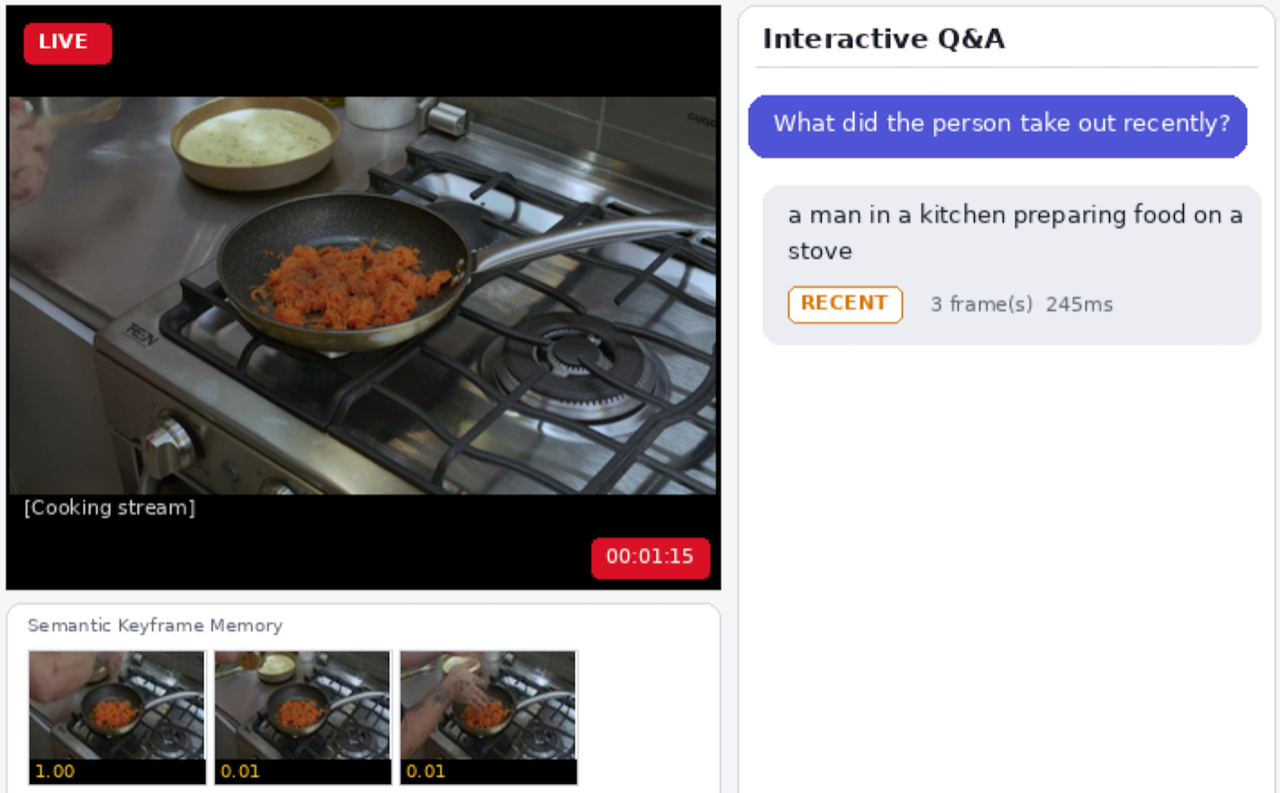
\includegraphics[width=\linewidth]{figures/qual_recent.pdf}
    \caption{Recent-scope query on a cooking stream.}
    \label{fig:qual-recent}
  \end{subfigure}
  \hfill
  \begin{subfigure}{0.32\linewidth}
    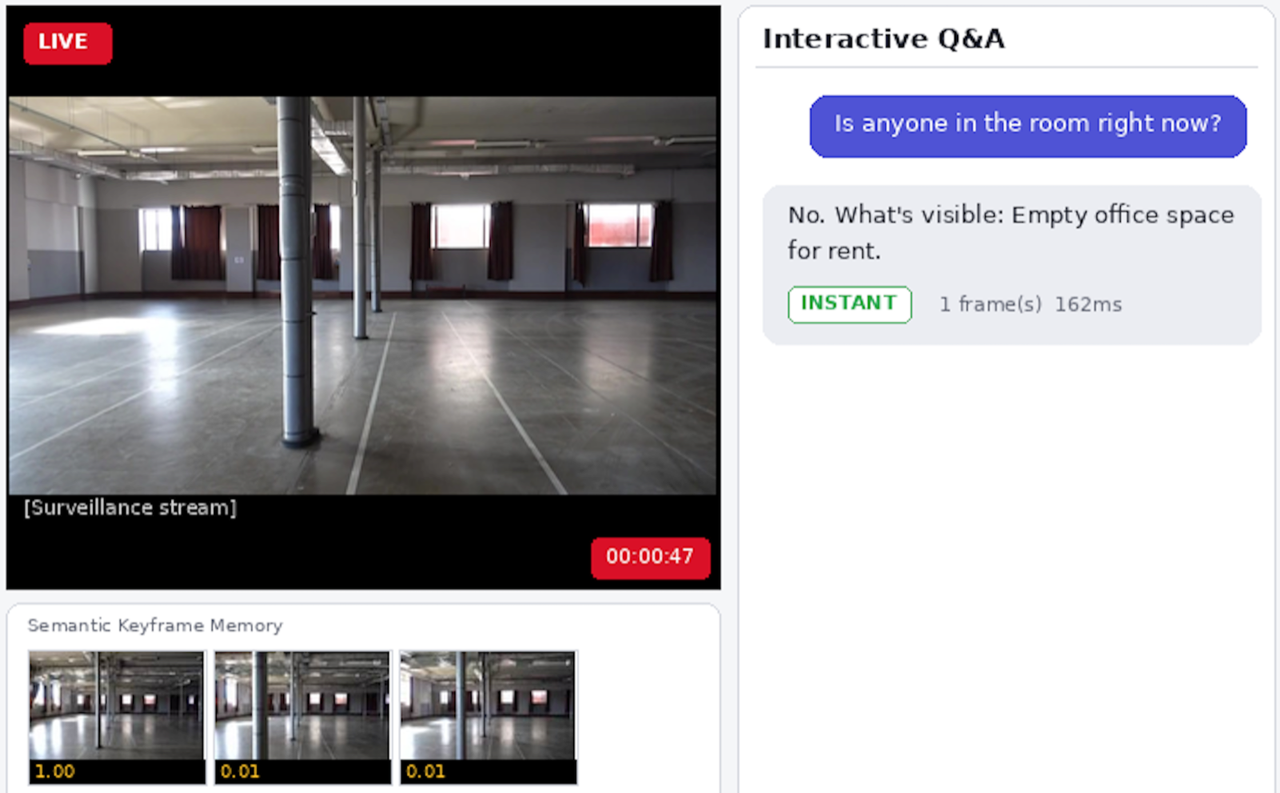
\includegraphics[width=\linewidth]{figures/qual_instant.pdf}
    \caption{Instant-scope query on a surveillance feed.}
    \label{fig:qual-instant}
  \end{subfigure}
  \hfill
  \begin{subfigure}{0.32\linewidth}
    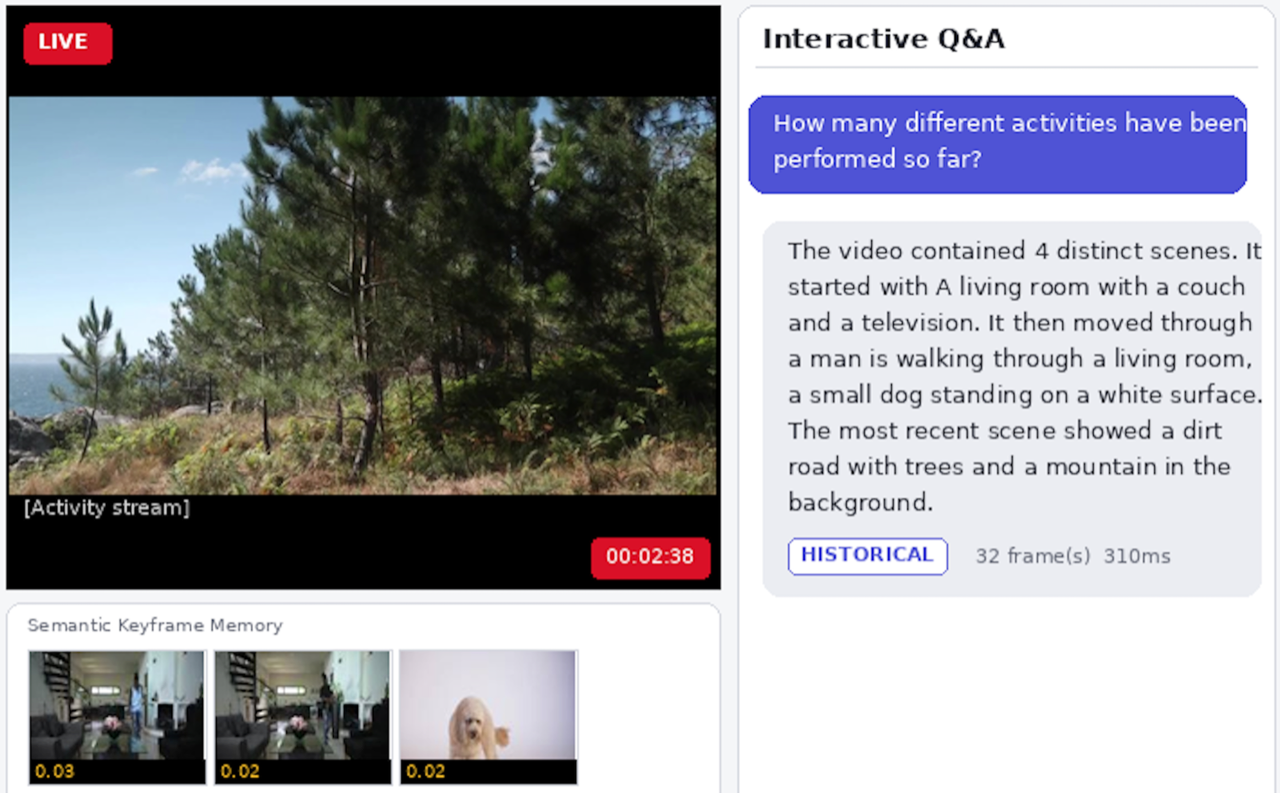
\includegraphics[width=\linewidth]{figures/qual_historical.pdf}
    \caption{Historical-scope query on an activity stream.}
    \label{fig:qual-historical}
  \end{subfigure}
  \caption{\textbf{Qualitative examples.} Three representative queries spanning all temporal scopes. Each panel shows the live video frame (top-left), SKM filmstrip (bottom-left), and the Q\&A interaction with scope tag and latency (right). \ours routes each question to the correct time window and produces grounded answers.}
  \label{fig:qualitative}
\end{figure*}

\subsection{Qualitative Results}
\label{sec:qualitative}

\Cref{fig:qualitative} shows three demo queries, one per scope.
In~(a), \emph{``What did the person take out of the fridge?''} triggers \textsc{recent}; the SKM retrieves the last 30\,s of keyframes and the answer correctly identifies \emph{milk and cheese}.
In~(b), \emph{``Is anyone in the room right now?''} triggers \textsc{instant}; only the latest frame is used and the system answers \emph{``No, the room is currently empty.''}
In~(c), \emph{``How many different activities have been performed so far?''} triggers \textsc{historical} over a 15-minute stream. BLIP captions across 64 keyframes reveal three distinct activities; a FIFO buffer would have overwritten the early frames.

\paragraph{LiveQA-Bench examples.}
\Cref{fig:liveqa_examples} shows two additional LiveQA-Bench predictions.
A \textsc{historical} query on a 12-minute home stream (\emph{``Did anyone leave the room earlier?''}) correctly identifies a departure event retained as a high-novelty frame.
A \textsc{recent} query on a 20-minute kitchen stream (\emph{``What was just placed on the counter?''}) retrieves the last 30\,s and identifies a cutting board and vegetables.

\begin{figure}[t]
  \centering
  
\includegraphics[width=\linewidth]{figures/qual_liveqa_examples.pdf}
  \caption{\textbf{LiveQA-Bench predictions.} Two examples showing historical (top) and recent (bottom) scope routing on long simulated streams. Correct scope classification enables accurate answers even for events that occurred minutes earlier.}
  \label{fig:liveqa_examples}
\end{figure}
